\begin{figure}[!t]
    \centering
    \footnotesize
    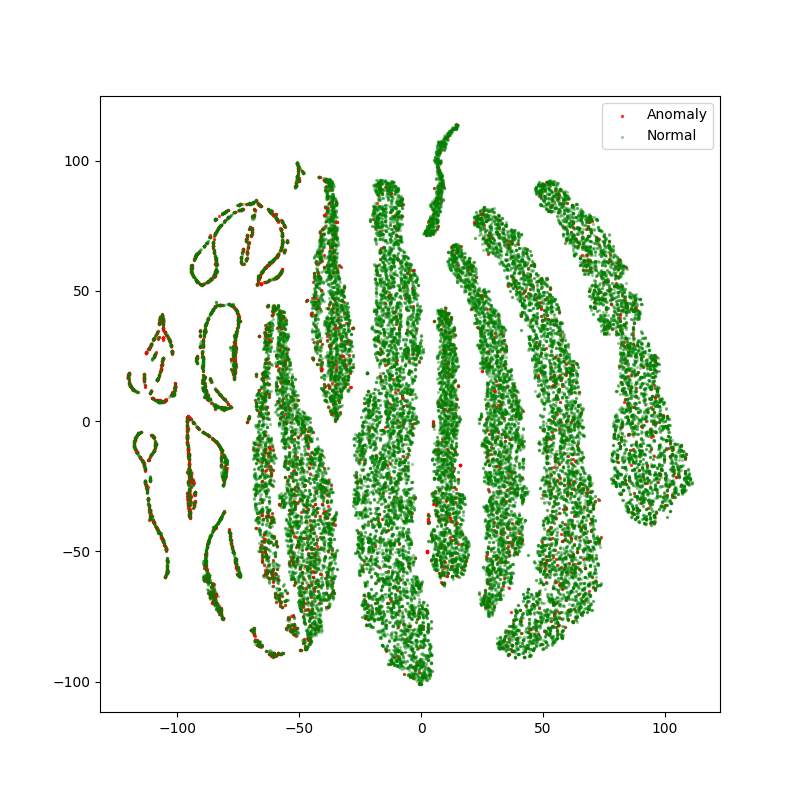
\includegraphics[width=0.75\linewidth,trim={1cm 1cm 1cm 1cm},clip]{../../results/figures/raw_tsne.png}
    \caption{Two-dimensional t-SNE projection of the input feature space}
    \label{fig:tsne_input}
    \vspace{1mm}
    \begin{minipage}{\columnwidth}
        The projection exhibits class separability between normal and anomalous observations. The plot was obtained using the t-distributed stochastic neighbor embedding (t-SNE) algorithm with two output dimensions and a fixed random seed for reproducibility. The input data was imputed, transformed through bucketing or logarithmic scaling where appropriate, and subsequently encoded for modeling. The scatter plot displays the embedded features color-coded by label, where anomalies (\texttt{y} = 1) are plotted in red and normal samples (\texttt{y} = 0) in green. The embedding was computed using the \texttt{sklearn.manifold} module.
    \end{minipage}
\end{figure}